\documentclass[a4paper, 11pt]{article}
\usepackage[utf8]{inputenc}
\usepackage{mathtools}
\usepackage{amsmath}
\usepackage{titlesec}
\usepackage{amssymb}
\usepackage{gensymb}
\usepackage[catalan]{babel}
\usepackage[dvipsnames]{xcolor}
\usepackage[margin=1in]{geometry}
\usepackage[hidelinks]{hyperref}
\usepackage{fancyhdr}
\usepackage{graphicx}
\usepackage{cancel}
\usepackage{subcaption}
\usepackage{tabto}
\usepackage{subcaption}
\usepackage{tocloft}
\usepackage{float}
\usepackage[style=numeric-comp, sorting=none]{biblatex}
\bibliography{bib.bib}
\newcommand{\figuretag}[1]{%
  \addtocounter{figure}{-1}%
  \renewcommand{\thefigure}{#1}%
}


\setcounter{tocdepth}{1}
\renewcommand{\cftdot}{.}
\pagestyle{fancy}
\lhead{Treball d'Astrofísica}
\rhead{}

\begin{document}
\begin{figure}
    \centering
    
\includegraphics[width=0.6\textwidth]{images/Logo_uab.png}
   % \caption{Caption}%
    \label{uab}
\end{figure}

\title{{\textbf{\Large LLIURAMENT D'INTRODUCCIÓ A L'ASTROFÍSICA: UNDERSTANDING ANALEMMAS
}\\}

\vspace{12mm}

{\large Facultat de ciències}\\
{\large Introducció a l'Astrofísica}}

\author{\textbf{Reina Delgado, Airan (1670808)}}
\date{}


\maketitle

\vspace{70mm} \title{\textbf{\Large NOTA:}}


%%%%%%%%%%%%%%%%%%%%%%%%%%%%%%%%%%%
%%%%%%%%%%%%%%%%%%%%%%%%%%%%%%%%%%%

    \vspace{4mm} 
    \noindent En la realització del treball s'ha generat contingut pròpi que, amb intenció de simplificar el treball del corrector, s'ha agrupat en un Github. El link del Github és el següent: \url{https://github.com/AiranReina/treball_astro/tree/main}. Allà es troba un README.md que resumeix els arxius d'interés en el treball i les seves localitzacions. 
    \newpage

%%%%%%%%%%%%%%%%%%%%%%%%%%%%%%%%%%%
%%%%%%%%%%%%%%%%%%%%%%%%%%%%%%%%%%%
%%%%%%%%%%%%%%%%%%%%%%%%%%%%%%%%%%%
%%%%%%%%%%%%%%%%%%%%%%%%%%%%%%%%%%%
%%%%%%%%%%%%%%%%%%%%%%%%%%%%%%%%%%%

\section*{EXERCICI 1}

\noindent Un analema és la corba que descriu el Sol al cel si s’observa des d'un lloc fix, a la mateixa hora del dia, cada dia de l’any. L’analema forma una corba que, aproximadament sol ser, una forma de vuit o lemniscata. Es poden observar analemes en altres planetes del Sistema Solar, però tenen una forma diferent de la que s’observa a la Terra, podent arribar a ser corbes diferents d’un vuit (a Mart és molt semblant a una gota d’aigua), tot i que tenen com a característica comuna que sempre són tancades \cite{DEFINICIO_ANALEMA}. Un exemple d’analema és el que es pot observar a la figura \ref{fig:analema}.

\begin{figure}[h!]
    \centering
    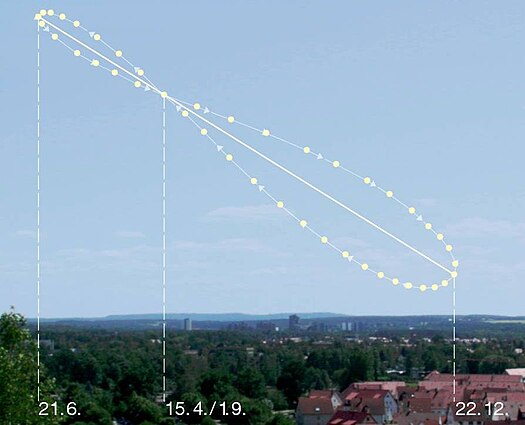
\includegraphics[width=0.6\textwidth]{images/analema.png}
    \caption{Analema solar per un observador a l'hemisfèri nord. Font: Wikipedia \cite{DEFINICIO_ANALEMA}.}
    \label{fig:analema}
\end{figure}
\vspace{10mm}
\hrule\
\vspace{5mm}


%%%%%%%%%%%%%%%%%%%%%%%%%%%%%%%%%%%
%%%%%%%%%%%%%%%%%%%%%%%%%%%%%%%%%%%

\section*{EXERCICI 2}
\noindent  En coordenades equatorials, un objecte en la bòveda celeste es pot localitzar amb les coordenades "ascensió recta" ($\alpha$ o $ra$) i "declinació" ($\delta$ o $dec$). El pla des d'ón es defineixen les coordenades és l'equador celestial, que és el pla perpendicular a l'eix de rotació de la Terra coincident amb l'equador terrestre. La declinació és l'angle entre l'equador i el cos celeste i, l'ascensió recta, és l'angle (En hores) del cos al voltant de l'equador celestial. El moviment vertical aparent del Sol en l'analema prové del canvi en la declinació solar al llarg de l'any degut a que la Terra orbita al voltant del Sol amb l'eix de rotació inclinat uns 23.5 graus respecte al pla de l'òrbita \cite{ANALEMA_WIKI}.
\vspace{10mm}
\hrule\
\vspace{5mm}

%%%%%%%%%%%%%%%%%%%%%%%%%%%%%%%%%%%
%%%%%%%%%%%%%%%%%%%%%%%%%%%%%%%%%%%

\section*{EXERCICI 3}
\noindent El moviment transversal (Est-Oest) aparent del Sol en l'analema prové del canvi no uniforme de l'ascensió recta solar al llarg de l'any degut als efectes combinats de la inclinació de l'eix de rotació de la Terra i l'eccentricitat de l'òrbita terrestre (Que genera una variació de la velocitat orbital de la Terra al llarg de l'any) \cite{ANALEMA_WIKI}. Aquests dos efectes generen una desigualtat en el moviment aparent del Sol al llarg de l’equador celeste, de manera que el Sol no arriba cada dia al meridià a la mateixa hora segons un rellotge mitjà. Aquest desfasament es quantifica mitjançant l’equació del temps, que expressa la diferència entre el temps solar veritable (Marcat per la posició real del Sol) i el temps solar mitjà (Definit per un moviment solar fictici uniforme) \cite{EQ_OF_TIME}.
\vspace{10mm}
\hrule\
\vspace{5mm}

%%%%%%%%%%%%%%%%%%%%%%%%%%%%%%%%%%%
%%%%%%%%%%%%%%%%%%%%%%%%%%%%%%%%%%%

\section*{EXERCICI 4}
\noindent Per resoldre aquest apartat es necesiten unes matemàtiques complexes i, com s'ha esmentat a l'enunciat de l'entrega, es pot fer us de IA i recursos web. En aquest cas, s'ha emprat com a guía els enllaços \cite{EQ_OF_CENTER}, \cite{E_ANOMALY} i \cite{M_EQ}, encara que els càlculs intermitjos són própis.

\vspace{2mm}

\noindent Començem, doncs, per entendre i definir els paràmetres de les órbites en moviments Keplerians. La posició d'un objecte celeste en el sistema solar es pot definir mitjançant la anomalía veritable $\nu$ (L'angle que escombra la recta que uneix el focus amb l'objecte des del periheli fins a la posició en la órbita real), la anomalía mitja $M$ (L'angle escombrat si l'objecte estigués en una órbita circular de radi $a$, el semieix major de la elípse) o la anomalía excèntrica $E$ (L'angle escombrat en la circunferència hipotètica si la coordenada $x$ és la real). Per trobar les relacions entre $M$ i $\nu$, serà interessant trobar primer les relacions d'ambdós paràmetres amb $E$, per després relacionarles entre sí. Un diagrama dels paràmetres restants es troba en la figura de l'esquerra de \ref{fig:esquema_orbites}.

\begin{figure}[h!]
    \centering
    \begin{subfigure}{0.45\textwidth}
        \centering
        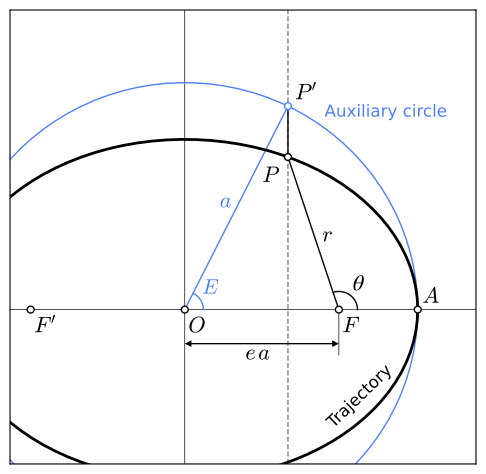
\includegraphics[width=\textwidth]{images/esquema_orbites.png}
        \caption{Esquema visual per entendre els paràmetres. Font: Wikipedia \cite{E_ANOMALY}.}
    \end{subfigure}
    \hspace{0.05\textwidth}
    \begin{subfigure}{0.45\textwidth}
        \centering
        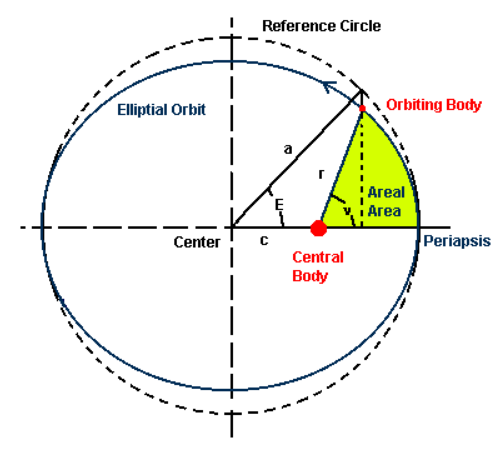
\includegraphics[width=\textwidth]{images/esquema_posicio.png}
        \caption{Esquema visual per entendre les diferents àrees necesàries en la demostració. Font: Bogan \cite{M_EQ}.}
    \end{subfigure}
    \caption{Esquemes necesàris per entendre la demostració}
    \label{fig:esquema_orbites}
\end{figure}

\noindent Per definició d'$E$, $cos(E) = \frac{x}{a}$. Sabem també que l'equació de la elipse és $\frac{x^2}{a^2} + \frac{y^2}{b^2} = 1$ i, com que el primer terme és $cos^2(E)$, el segón ha de ser $sin^2(E)$ per cumplir l'igualtat trigonomètrica $sin^2(x) + cos^2(x) = 1$. Aquestes dos relacions amb la definició d'excentricitat $\epsilon$ ens donen 3 relacions importants:

\begin{equation} \label{relacions_Eie}
    \boxed{\cos(E) = \cfrac{x}{a}} \hspace{5mm} \boxed{\sin(E) = \cfrac{y}{b}} \hspace{5mm} \boxed{\epsilon \equiv \sqrt{1-\cfrac{b^2}{a^2}}}
\end{equation}
\vspace{2mm}

\noindent Amb aquestes relacions, podem trobar una expresió que ens relacioni $E$ i $\nu$ per començar. Sabem que $cos(E) = \frac{x}{a} = \frac{\epsilon a + rcos(\nu)}{a}$, anem doncs a trobar una expressió per $r$ (Amb arguments geomètrics):

\begin{align*}
    r^2 &= y^2 + (\epsilon a - x)^2 = b^2 sin ^2(E) + (\epsilon a - acos(E))^2 = ...\\
    & \hspace{10mm} \left[ \epsilon ^2 = 1- \cfrac{b^2}{a^2} \hspace{2mm} \implies \hspace{2mm} b^2 = a^2 (1-\epsilon^2) \right] \\
    ... &= a^2 [(1-\epsilon^2)(1-cos^2(E)) + (\epsilon - cos(E))^2] = \\
    &= a^2 [1 - cos^2(E) -\epsilon ^2 + \epsilon ^2 cos^2(E) + \epsilon^2 + cos^2(E) -2\epsilon cos(E)] = \\
    &= a^2 [1 - 2\epsilon cos(E) + \epsilon^2 cos^2(E)] = a^2[1-\epsilon cos(E)]^2
\end{align*}

\noindent Tenint doncs una expressió per $r$, seguim amb el càlcul que estàvem fent abans i, després, per trobar una expressió $sin(E)$ en funció de $\nu$, apliquem la identitat trigonomètrica $sin^2(x) + cos^2(x) = 1$:

\begin{align*}
    &cos(E) = \cfrac{\epsilon a + [a(1-\epsilon cos(E))] cos(\nu)}{a} = \epsilon + cos(\nu) - \epsilon cos(E) cos(\nu)\\
    &cos(E)[1+\epsilon cos(\nu)] = \epsilon + cos(\nu) \hspace{2mm} \implies \hspace{2mm} cos(E) = \cfrac{\epsilon + cos(\nu)}{1 + \epsilon cos(\nu)} \\
\end{align*}
\begin{align*}
    &sin(E) = \sqrt{1 - cos^2(E)} = \cfrac{\sqrt{[1+\epsilon cos(\nu)]^2 - [\epsilon + cos(\nu)]^2}}{1+\epsilon cos(\nu)} = \\
    &\cfrac{\sqrt{1 + \epsilon^2 cos^2(\nu) - \epsilon^2 - cos^2(\nu)}}{1+\epsilon cos(\nu)} = \cfrac{\sqrt{[1-cos^2(\nu)][1-\epsilon^2]}}{1+\epsilon cos(\nu)}
\end{align*}
\vspace{2mm}
\begin{equation} \label{relacions_Enu}
    \implies \hspace{5mm} \boxed{cos(E) = \cfrac{\epsilon + cos(\nu)}{1 + \epsilon cos(\nu)}} \hspace{5mm} \boxed{sin(E) = \cfrac{\sqrt{1-\epsilon^2}sin(\nu)}{1 + \epsilon cos(\nu)}}
\end{equation}
\vspace{2mm}

\noindent Ara que tenim les relacions $E(\nu)$, anem a trobar la relació $M(E)$. Aquesta relació es troba directament de la segona llei de Kepler. La segona llei de Kepler ens diu que "\textit{El segment que uneix un planeta amb el Sol escombra arees iguals per temps iguals}". Per intentar trobar la relació $M(E)$, necesitem definir 3 àrees diferents i aplicar la segona llei de Kepler. Si observem la imatge de la dreta de la figura \ref{fig:esquema_orbites}, definim l'àrea de referència ($A_{ref}$) com l'àrea que escombra el radi de la circunferència hipotètica que forma un angle $E$; definim l'àrea auxiliar ($A_{aux}$) com l'àrea escombrada en l'elipse pel segment que uneix el centre amb l'objecte real; finalment, definim l'àrea real ($A_{real}$) com l'àrea escombrada en l'elipse pel segment que uneix el focus amb l'objecte real (Es veu sombrejat en verd en la imatge esmentada). Definint aquestes àrees, tenim:

\begin{align*}
    &A_{ref} = \textit{(Fracció Angular) ·} \hspace{1mm}  A_{cercle} = \cfrac{E}{2\pi}\pi a^2 = E\cfrac{a^2}{2} \\
    &A_{aux} = A_{ref} \cfrac{b}{a} = A_{ref} \sqrt{1-\epsilon^2} = E\cfrac{a^2}{2} \sqrt{1-\epsilon^2} \\
    &\left[ A_{aux} - A_{real} = A_{triangle}\cfrac{b}{a} = \cfrac{[base][altura]}{2}\cfrac{b}{a} = \cfrac{[a][a\epsilon sin(E)]}{2} \sqrt{1-\epsilon ^2} \right] \\
    &A_{real} = A_{aux} - A_{triangle} = \cfrac{a^2}{2} \sqrt{1-\epsilon^2} [E - \epsilon sin(E)] \\
\end{align*}

\noindent La segona llei de Kepler ens diu que $\frac{A}{t} = ct$ $\implies$ $A = Kt$ $\forall t$, en especial és vàlid per $t=T$, que és l'àrea de l'elipse sencera, $A = \pi ab = \pi a^2 \sqrt{1-\epsilon^2} = KT$. Per tant, podem escriure:

\begin{align*}
    &KT = \pi a^2 \sqrt{1-\epsilon^2} \hspace{2mm} \implies \hspace{2mm} K = \cfrac{\pi a^2}{T} \sqrt{1-\epsilon^2} \\
    &Kt = \cfrac{\pi a^2}{T} \sqrt{1-\epsilon^2} t = A_{real} = \cfrac{a^2}{2} \sqrt{1-\epsilon^2} [E - \epsilon sin(E)] \hspace{2mm} \implies \hspace{2mm} \cfrac{2\pi t}{T} = E - \epsilon sin(E) \\
\end{align*}

\noindent Com sabem, $M$ és la posició hipotètica en l'órbita circular. Com l'órbita és circular, per la primera llei de Kepler sabem que el Sol s'hauría de trobar al centre i, per tant, la velocitat angular és constant. Per aquesta raó, podem definir $M$ com l'angle escombrat en el temps $t$, és a dir, $M \equiv 2\pi \cfrac{t}{T}$, per tant:

\begin{equation} \label{relacio_ME}
    \boxed{M(E) = E - \epsilon sin(E)}
\end{equation}
\vspace{2mm}

\noindent Ara, ja tenim totes les relacions necesàries per trobar $M(\nu)$. Per trobar aquesta relació, només hem de substituir la relació $E(\nu)$(Eq. \ref{relacions_Enu}) del $sin(E)$ en la relació $M(E)$ (Eq. \ref{relacio_ME}). Un cop fet això, trobem la relació no trascendental següent:

\vspace{2mm}
\begin{equation} \label{relacio_Mnu}
    \boxed{ M(\nu) = arcsin \left[ \cfrac{\sqrt{1-\epsilon ^2} sin(\nu)}{1 + \epsilon cos(\nu)} \right] - \epsilon \cfrac{\sqrt{1-\epsilon ^2} sin(\nu)}{1 + \epsilon cos(\nu)} }
\end{equation}
\vspace{2mm}

\noindent Com es pot observar, trobar la relació inversa $\nu(M)$ es complica bastant. En el moviment Keplerià, les coordenades del cos celeste es repeteixen de manera periòdica en cada òrbita, fet que permet descriure-les mitjançant sèries periòdiques en funció de variables angulars creixents. L’anomalia mitjana $M$, que creix linealment amb el temps, és especialment útil perquè permet expressar altres variables orbitals en funció del temps. L’anomalia veritable $\nu$, tot i ser analítica respecte de $M$, no és una funció entera i té un radi de convergència limitat si s’expressa com a sèrie de potències. Tanmateix, pel fet de ser una funció periòdica, es pot expandir en una sèrie de Fourier que convergeix globalment. Els coeficients d’aquesta sèrie depenen d'$\epsilon$ i s’expressen mitjançant funcions de Bessel del primer tipus. De forma genèrica, la serie que aproxima la funció $\nu(M)$ és:

\begin{equation*}
    \nu(M) = M + 2\sum_{s=1}^{\infty} \cfrac{1}{s} \left[ J_s(s\epsilon) + \sum_{p=1}^{\infty} e^{-p}[1-\sqrt{1-\epsilon^2}]^p[J_{s-p}(s\epsilon) - J_{s+p}(s\epsilon)] \right] sin(sM)
\end{equation*}
\vspace{2mm}

\noindent Si expandim cadascuna de les funcions de Bessel i aproximem per $\epsilon \to 0$ (Que és bona aproximació considerant que per la Terra $\epsilon \approx 0.0167$), podem trobar una aproximació de la funció $\nu(M)$ que és vàlida per a qualsevol valor de $M$. Aquesta aproximació queda com:

\vspace{2mm}
\begin{equation} \label{aproximacio_Mnu}
    \boxed{  \nu(M) \simeq M + 2\epsilon sin(M) + \cfrac{5}{4} \epsilon ^2 sin(2M)  }
\end{equation}\
\vspace{2mm}

\noindent Ón hem aproximat per sota d'ordre $\epsilon^3$. La demostració explícita de la versió aproximada de $\nu(M)$ és bastant complexe i requereix matemàtiques extenses y avançades. Com s'ha dit a l'inici d'aquest exercici, s'han emprat diversos recursos com a guía. En específic, per aquesta part final, s'ha emprat la referència \cite{EQ_OF_CENTER} de la Wikipedia. Per trobar una expresió de major ordre, es poden trobar els termes d'ordre superior en la referència esmentada.

\vspace{2mm}

\noindent Finalment, per completitud, cal esmentar que la diferència $\nu - M$ és la quantitat anomenada "Equació de centre". Amb l'aproximació feta, l'equació de centre és  $C(M) \simeq 2\epsilon sin(M) + \frac{5}{4} \epsilon ^2 sin(2M)$. Aquesta quantitat és un paràmetre clau a l'hora de trobar la "Equació de temps", que ens permetrà graficar l'analema solar en exercicis propers.

\vspace{10mm}
\hrule\
\vspace{5mm}

%%%%%%%%%%%%%%%%%%%%%%%%%%%%%%%%%%%
%%%%%%%%%%%%%%%%%%%%%%%%%%%%%%%%%%%

\section*{EXERCICI 5}
\noindent L’equació del temps descriu la discrepància entre dos tipus de temps solar. Aquests dos temps són el temps solar aparent, que segueix directament el moviment del Sol, i el temps solar mitjà, que segueix un Sol teòric amb un moviment uniforme al llarg de l’equador celeste. El temps solar aparent es pot obtenir mesurant la posició actual (angle horari) del Sol, tal com indica (amb precisió limitada) un rellotge de sol. El temps solar mitjà, per al mateix lloc, seria el temps indicat per un rellotge regular ajustat de manera que, al llarg de l’any, les seves diferències respecte al temps solar aparent tinguin una mitjana de zero.

\vspace{2mm}

\noindent L’equació del temps presenta dues oscil·lacions amb forma d’ona sinusoïdal perquè hi ha dues causes físiques independents que afecten el moviment aparent del Sol respecte al temps solar mitjà. La primera és l’excentricitat de l’òrbita terrestre: com que l’òrbita de la Terra és el·líptica, la seva velocitat orbital varia al llarg de l’any. Aquesta variació provoca una desviació periòdica en la posició del Sol aparent, amb una ona sinusoïdal de període anual. La segona causa és la inclinació de l’eix de rotació de la Terra respecte al pla de la seva òrbita (la eclíptica). Aquest angle d’uns $\sim 23.5\degree$ fa que el moviment aparent del Sol al llarg de l’equador celeste no sigui uniforme, i això introdueix una segona variació també de tipus sinusoïdal, però amb el doble de freqüència angular. El efecte de la doble freqüència prové de que, en projectar el sol sobre el pla eclíptic celeste, ens dona una expresió de la forma $tan(\alpha) = cos(\sim 23.5 \degree) tan(\lambda)$, on $\alpha$ és l'ascensió recta i $\lambda$ és la longitud eclíptica. Quan expandim la funció $\alpha(\lambda)$ en aquesta expressió, trobem que s'aproxima a una serie de Fourier truncada de forma que queda $\alpha(\lambda) = \lambda - Csin(2\lambda) + ...$, ón $C$ és una constant.

\vspace{2mm}

\noindent La forma general de l'equació, trobada teòricament, és $\Delta t_{AM} \approx Asin(\omega t) + Bsin(2\omega t)$. En la literatura es troba una expressió on s'han aproximat experimentalment els valors de $A$, $B$ i $\omega$, que és \cite{EQ_OF_TIME}:

\begin{equation} \label{eq_time}
    \boxed{\Delta t_{AM}(y,d) = -7.659sin[D(y,d)] + 9.863 sin[2D(y,d) + 3.5932] \hspace{1mm} [minuts]} \hspace{5mm} \text{tal que:}
\end{equation}
\begin{equation*}
    D(y,d) = 6.24004077 + 0.01720197[365(y-2000) + d] \hspace{5mm} \text{(Ón $d$ és el dia de l'any $y$)}
\end{equation*}
\vspace{2mm}

\noindent Aquesta expressió es pot avaluar per l'any 2025 si substituim aquest valor en la funció auxiliar $D(y,d)$. Aquesta funció auxiliar queda doncs com:

\begin{equation} \label{D_2025}
    \boxed{D(2025,d) \equiv D(d) = 163.3155293 + 0.01720197d}
\end{equation}
\vspace{2mm}

\noindent És interessant observar com l'equació del temps està relacionada directament amb el temps sideral aparent o, simplement, el temps sideral ($T_{sideral}$). Mentre que el temps solar es basa en la rotació de la Terra en relació amb el Sol, el temps sideral es basa en la rotació de la Terra respecte a les estrelles fixes del cel. Un dia sideral té una durada de 23 hores, 56 minuts i 4 segons, mentre que un dia solar, que és el temps que mesuren els rellotges habituals, té una durada de 24 hores. Aquesta diferència es deu al fet que la Terra, a mesura que rota sobre el seu eix, també es mou una mica en la seva òrbita al voltant del Sol, i per tant necessita fer una mica més de rotació per tornar a situar el Sol en la mateixa posició al cel.

\vspace{2mm}

\noindent Per definició, l'equació del temps és $EoT = t_{\text{aparent}} - t_{\text{mitjà}} \equiv GHA - GMHA$. $GHA$ significa "Greenwich Hour Angle" i $GMHA$ "Greenwich Mean Hour Angle". $GMHA \equiv UT - \text{offset}$, on l'\textit{offset} és el temps mig solar quan el Sol està en el meridià de Greenwich, és a dir, les 12h (migdia solar mitjà). D'altra banda, si seguim les definicions dels angles de l'esfera celeste, $GHA = GAST - \alpha$, on $GAST$ és el "Greenwich Apparent Sidereal Time" i $\alpha$ és l'ascensió recta. Si juntem totes les relacions, ens dona una expressió que relaciona directament l'equació del temps amb el temps sideral.

\begin{equation}
    EoT = GAST - \alpha - UT + offset
    \label{eq:EoT_ST}
\end{equation}

\vspace{10mm}
\hrule\
\vspace{5mm}

%%%%%%%%%%%%%%%%%%%%%%%%%%%%%%%%%%%
%%%%%%%%%%%%%%%%%%%%%%%%%%%%%%%%%%%

\section*{EXERCICI 6}

\noindent Per realitzar aquest exercici, s'ha escrit un script en Python que es pot trobar al GitHub del treball. L'arxiu de l'script es diu \texttt{analema.py}. El codi calcula la posició del Sol [en coordenades horitzontals $(\text{Altitud}, \text{Azimut}) = (\text{alt}, \text{az})$ i en coordenades equatorials $(\text{Declinació}, \text{Ascensió Recta}) = (\text{dec}, \text{ra}) = (\delta, \alpha)$], calcula la diferència entre el temps solar mitjà i el temps solar aparent a partir de l’equació del temps i, finalment, genera la gràfica de l’analema solar vist des de Bellaterra. Els analemes generats es poden veure a la figura~\ref{fig:analema_terra}.


\begin{figure}[h!]
    \centering
    \begin{subfigure}{0.45\textwidth}
        \centering
        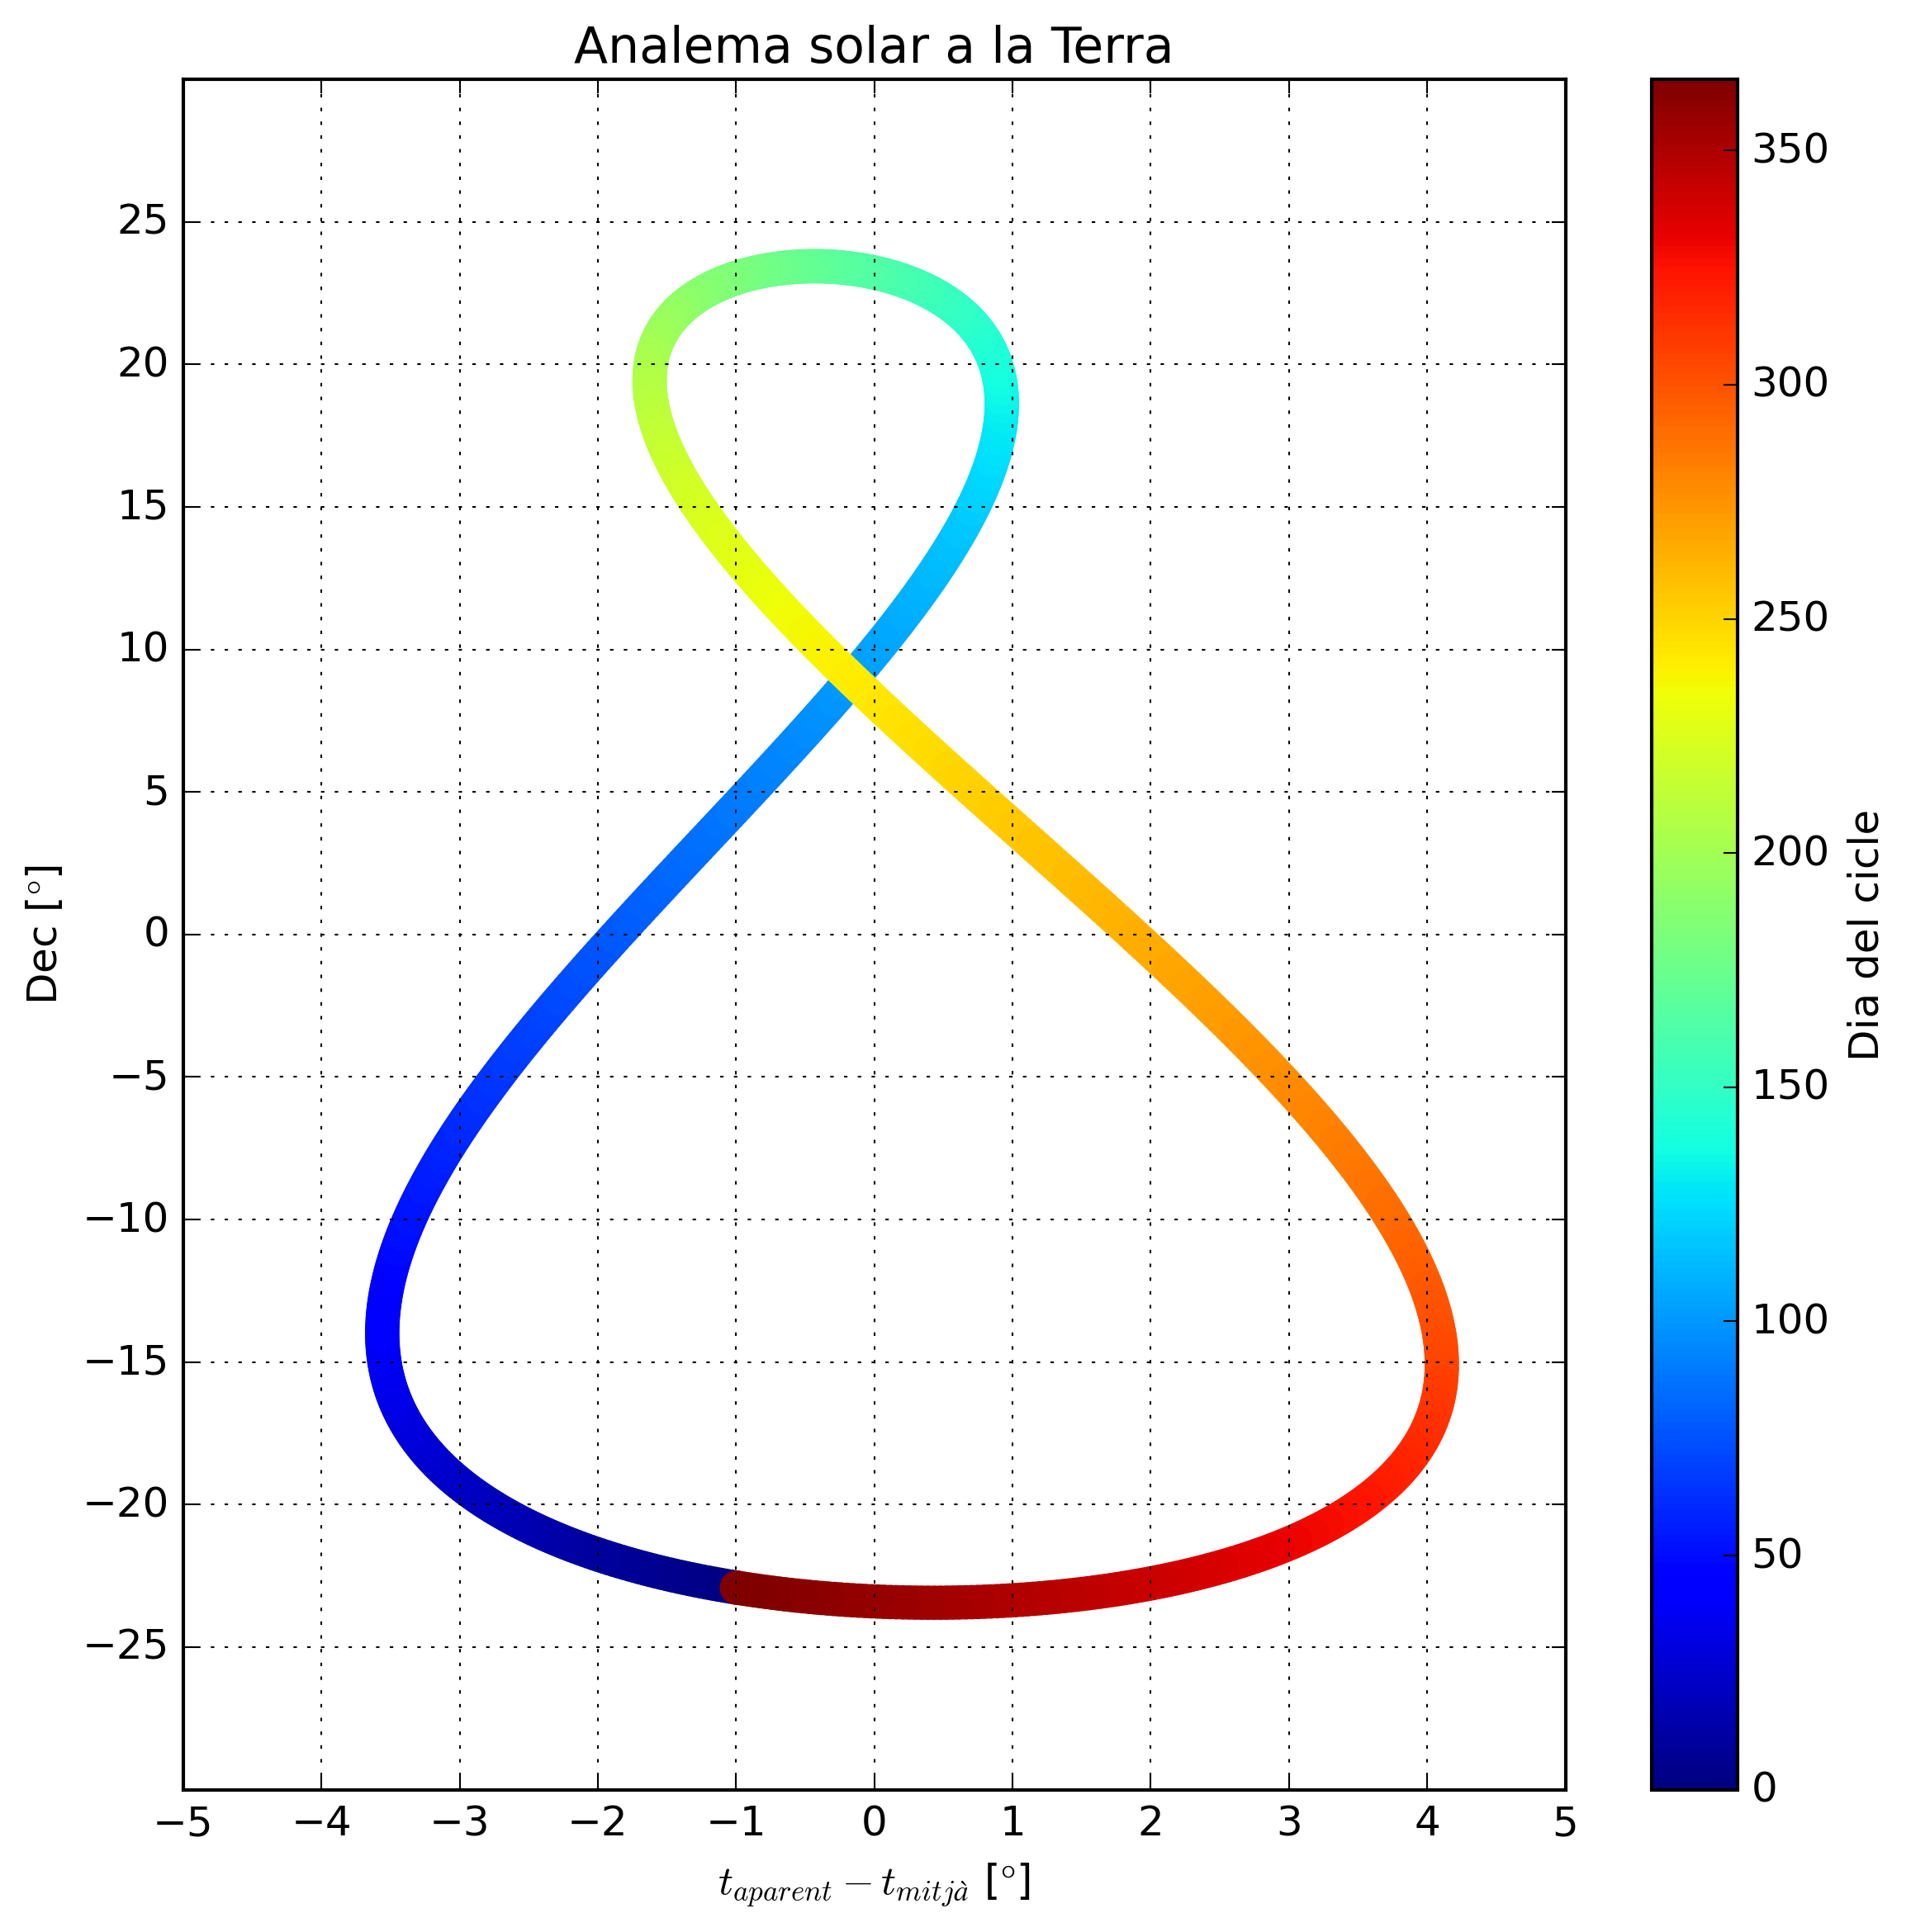
\includegraphics[width=\textwidth]{images/analema_dec_eot.png}
        \caption{Analema solar vist des de la Terra $dec$ ($EoT$). Font: Github del treball.}
    \end{subfigure}
    \hspace{0.05\textwidth}
    \begin{subfigure}{0.45\textwidth}
        \centering
        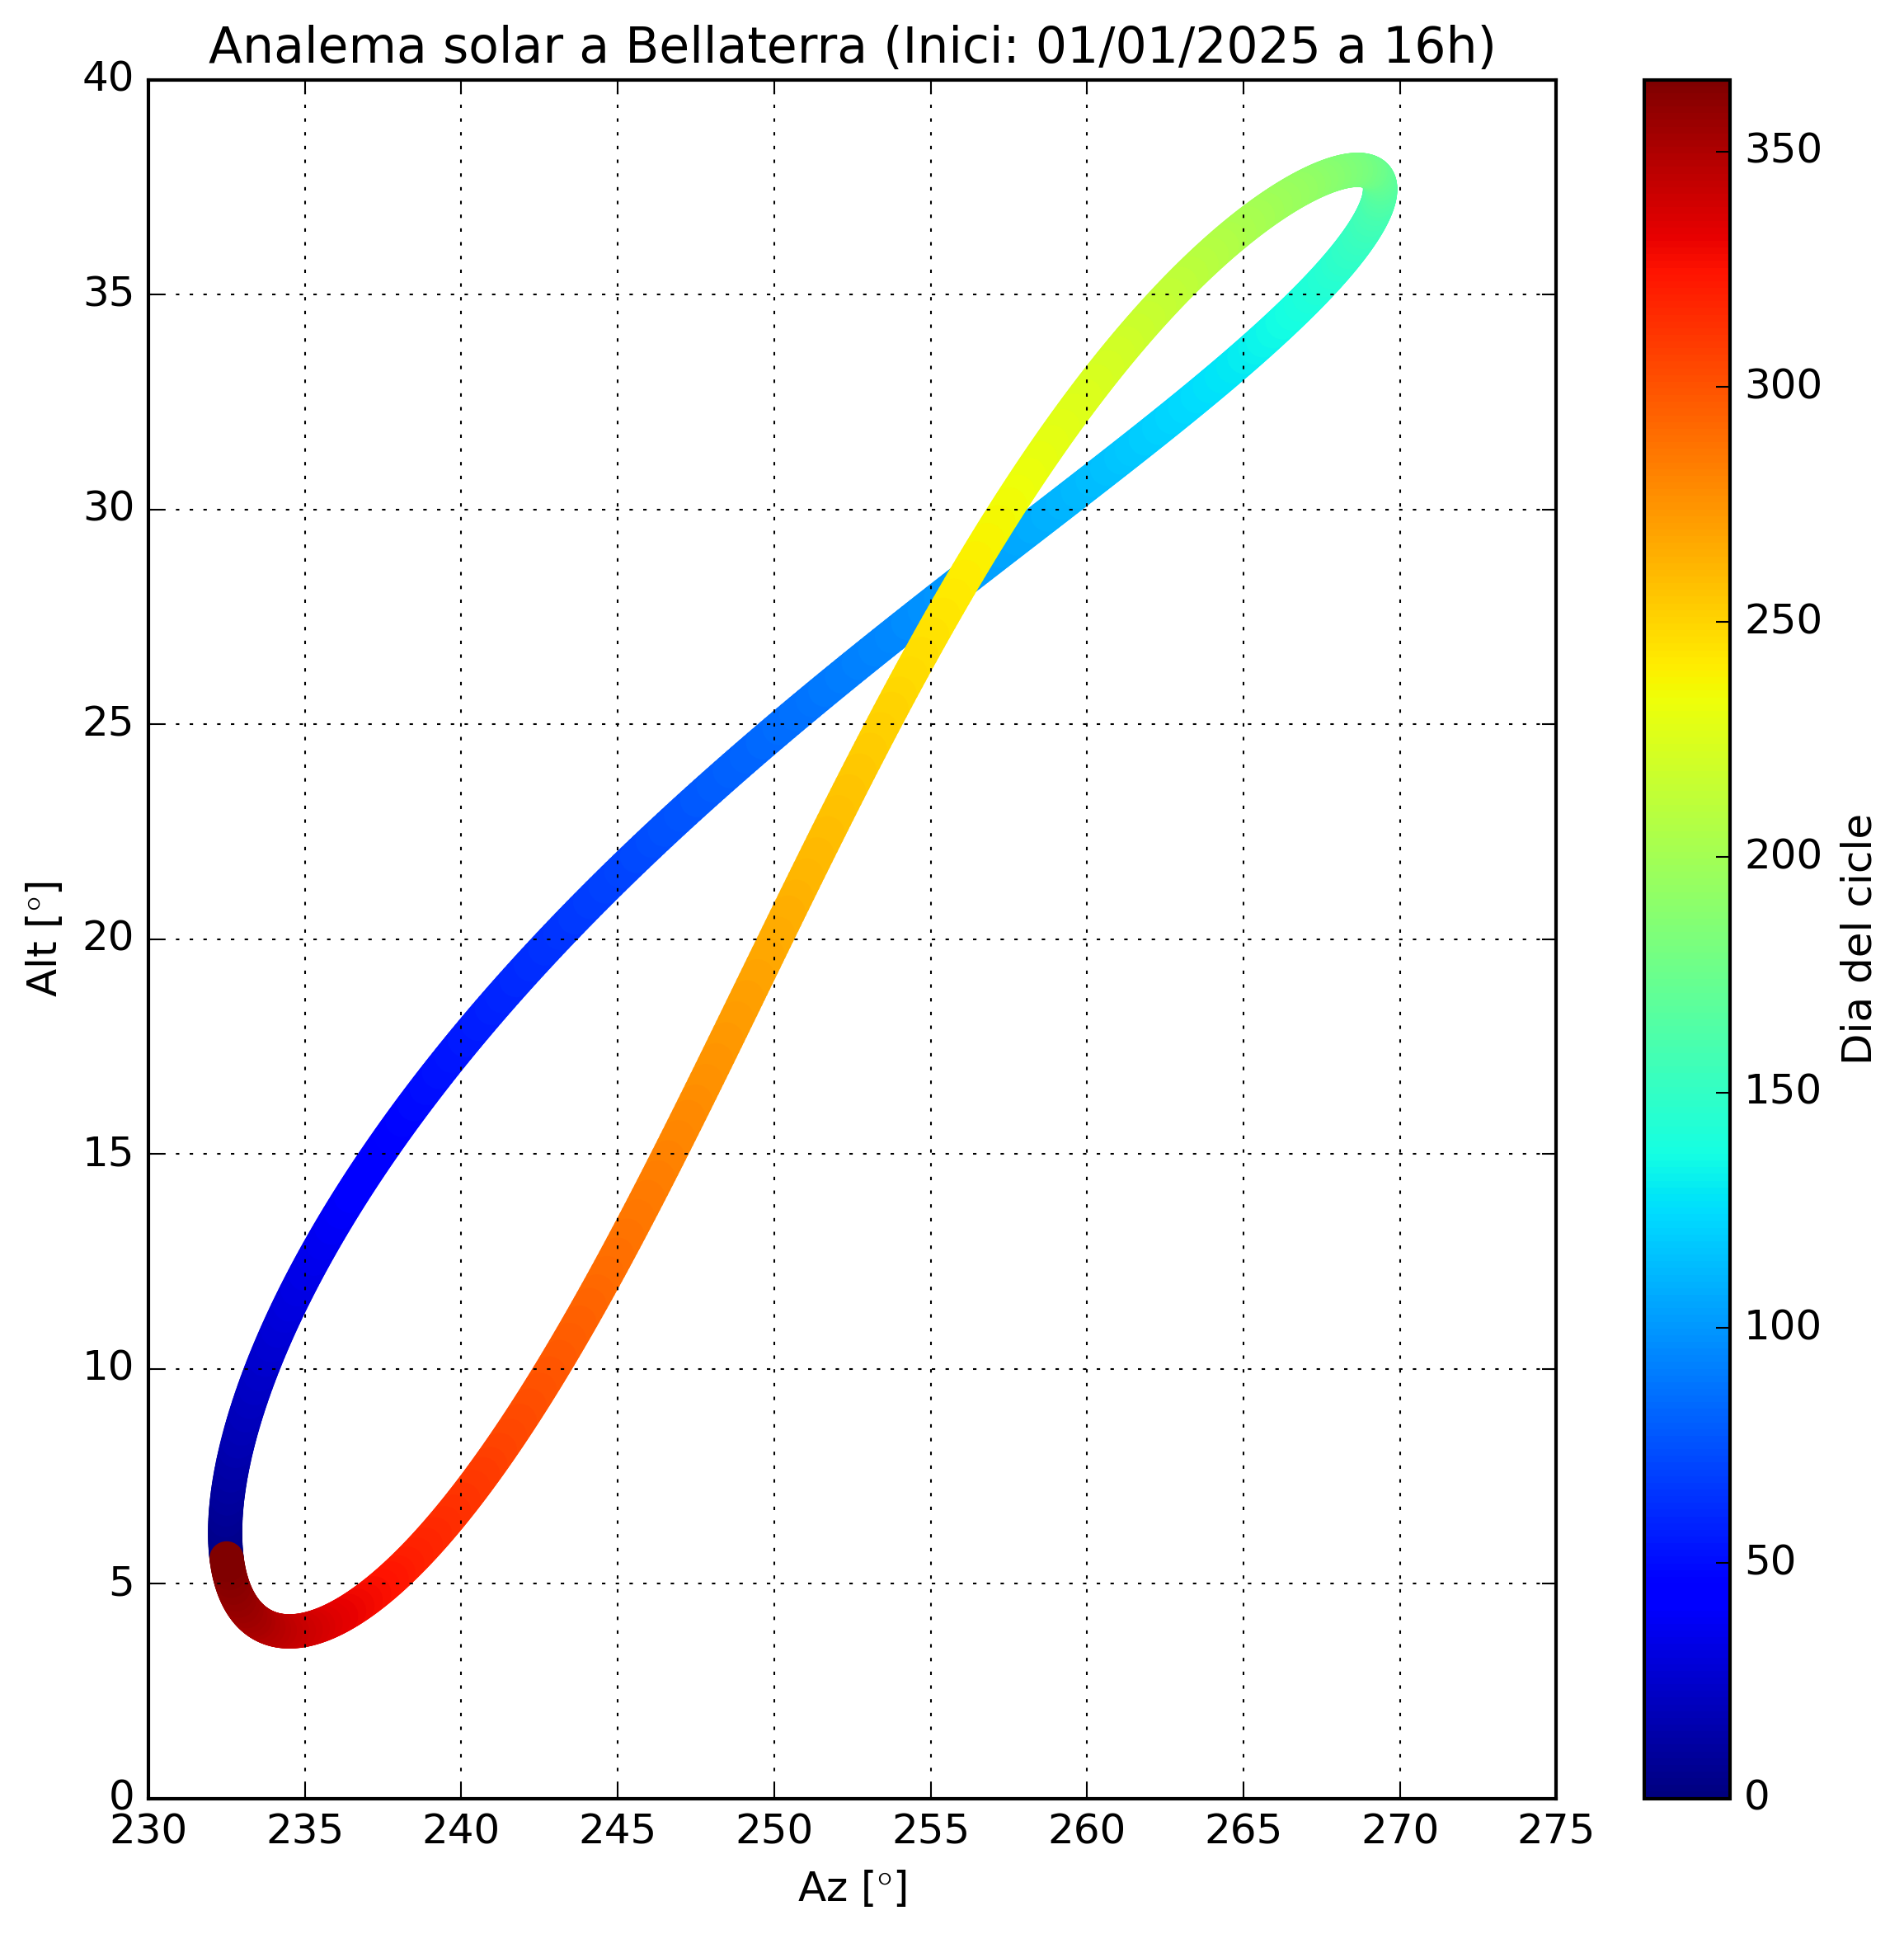
\includegraphics[width=\textwidth]{images/analema_alt_az.png}
        \caption{Analema solar vist des de la Terra $alt$ ($az$). Font: Github del treball.}
    \end{subfigure}
\caption{Analemes solars vist des de la Terra}
\label{fig:analema_terra}
\end{figure}
\vspace{2mm}

\noindent L'analema graficat en coordenades equatorials (O, equivalentment, la declinació en funció de l'equació del temps) és general del planeta Terra mentres que el graficat en coordenades horitzontals és vàlid per unes coordenades terrestres específiques (Les de Bellaterra en aquest cas). Aquesta observació és demostrable directament de la naturalesa d'ambdós coordenades, doncs les primeres són coordenades definides des de la própia Terra mentre que les segones es defineixen localment. Ambdúes representacions són vàlides, però la versió en coordenades horitzontals ens aporta informació extra doncs representa el que qualsevol observador pot analitzar a simple vista, té aplicacions pràctiques (Com als rellotges solars, concepte tractat en un exercici més endavant) i, a més, genera un grau de llibertat extra al anàlisi pel fet d'introduir variació dependent de les coordenades terrestres de l'observador. Degut a tot això, a partir d'ara sempre que es tracti el concepte d'analema, se suposarà intrínsicament la versió en coordenades horitzontals.

\vspace{2mm}

\noindent Finalment, és interessant analitzar l'analema que es troba en la paret de la facultat de ciències de l'UAB. En l'anunciat de l'entrega se'ns ha proporcionat la imatge sobre aquest analema. Aquesta es pot veure en la figura \ref{fig:analema_UAB}

\begin{figure}[h!]
    \centering
    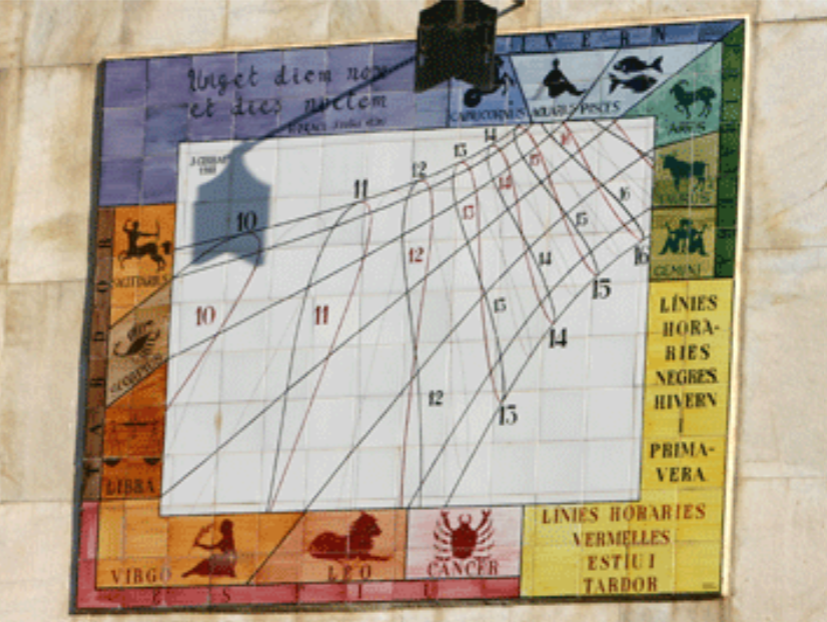
\includegraphics[width=0.6\textwidth]{images/analema_UAB.png}
    \caption{Analema solar a la paret de la facultat de ciències de l'UAB. Font: Enunciat Entrega.}
    \label{fig:analema_UAB}
\end{figure}
\vspace{2mm}

\noindent Com es pot observar, la placa conté un conjunt d'analemes. Cada analema està asociat a una hora del día, des de les 10h fins les 17h. A priori sembla que els analemes són correctes doncs tenen forma de "8", tenen un braç més llarg que l'altre, estan espaiats coherentment sabent que cada analema és l'adequat a una hora específica, etc. Igualment, és interessant realitzar un anàlisi més profund. En el mateix codi, s'ha generat també una figura com la que es pot veure a la entrada de la UAB. El resultat es pot veure en la imatge \ref{subfig:analema_simUAB}.

\begin{figure}[h!]
    \centering
    \begin{subfigure}{0.42\textwidth}
        \centering
        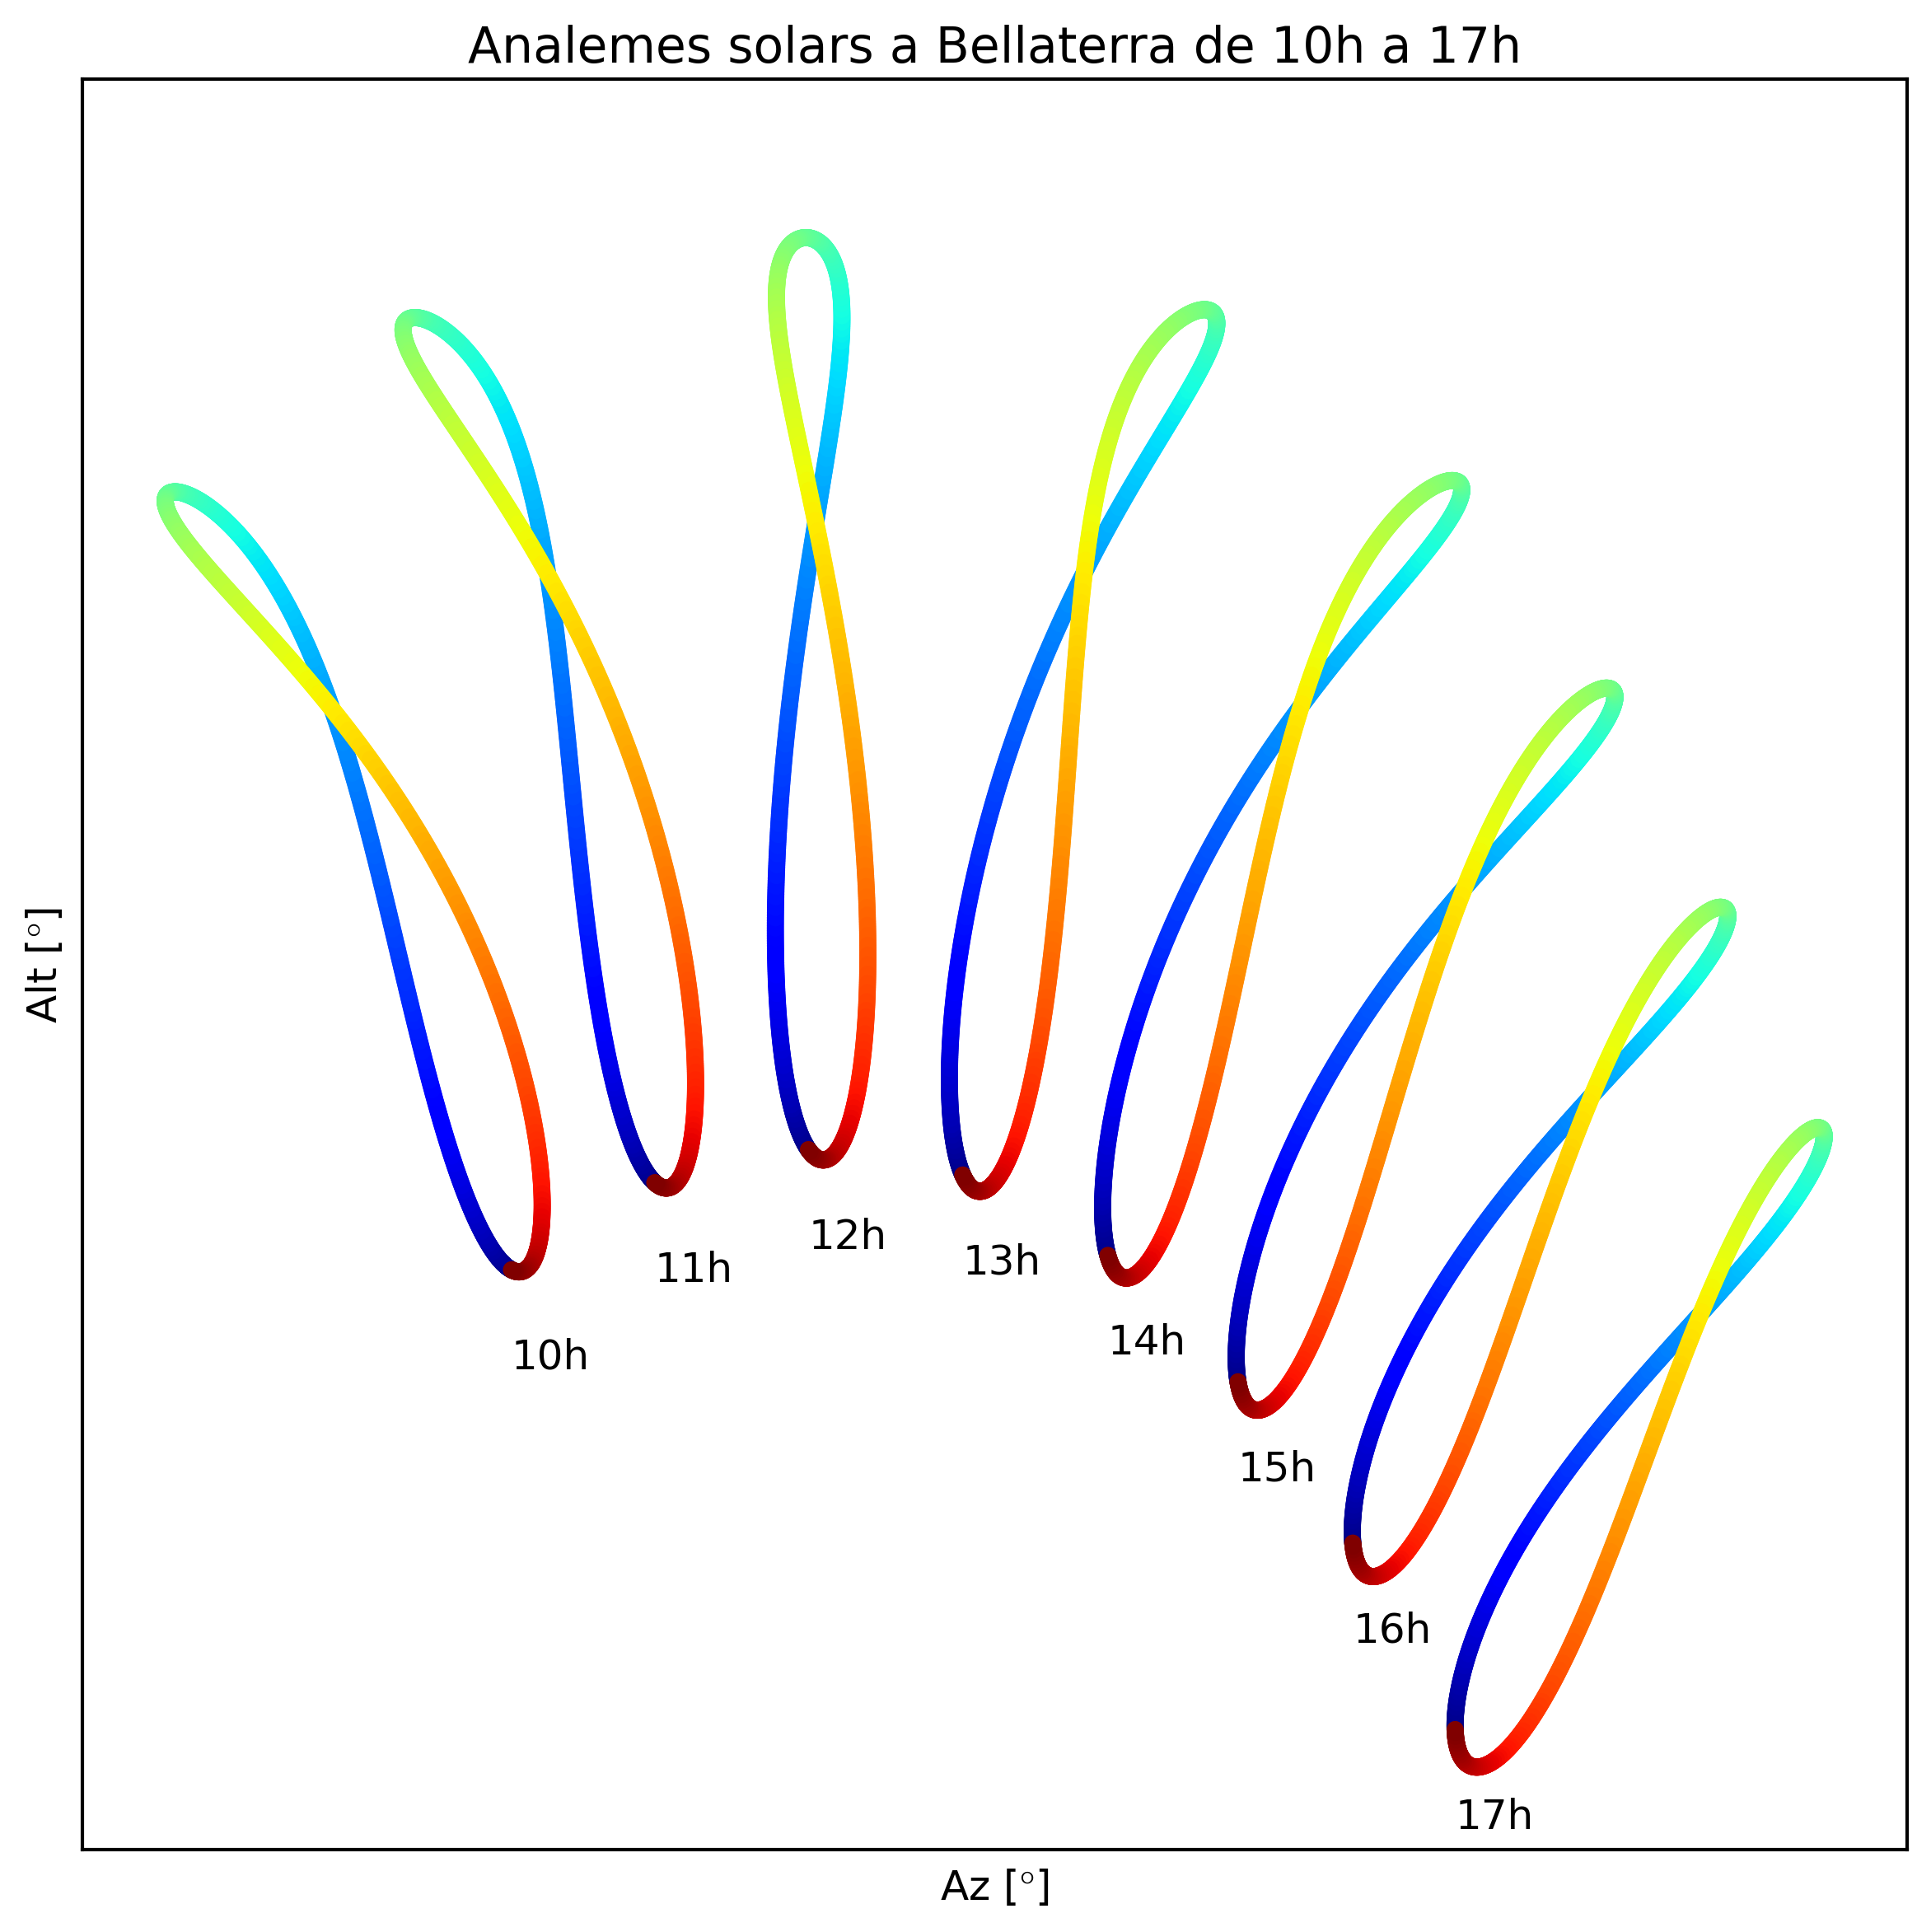
\includegraphics[width=\textwidth]{images/analema_simUAB.png}
        \caption{Analemes d'un conjunt d'hores vist des de la Terra. Font: Github del treball.}
        \label{subfig:analema_simUAB}
    \end{subfigure}
    \hspace{0.05\textwidth}
    \begin{subfigure}{0.48\textwidth}
        \centering
        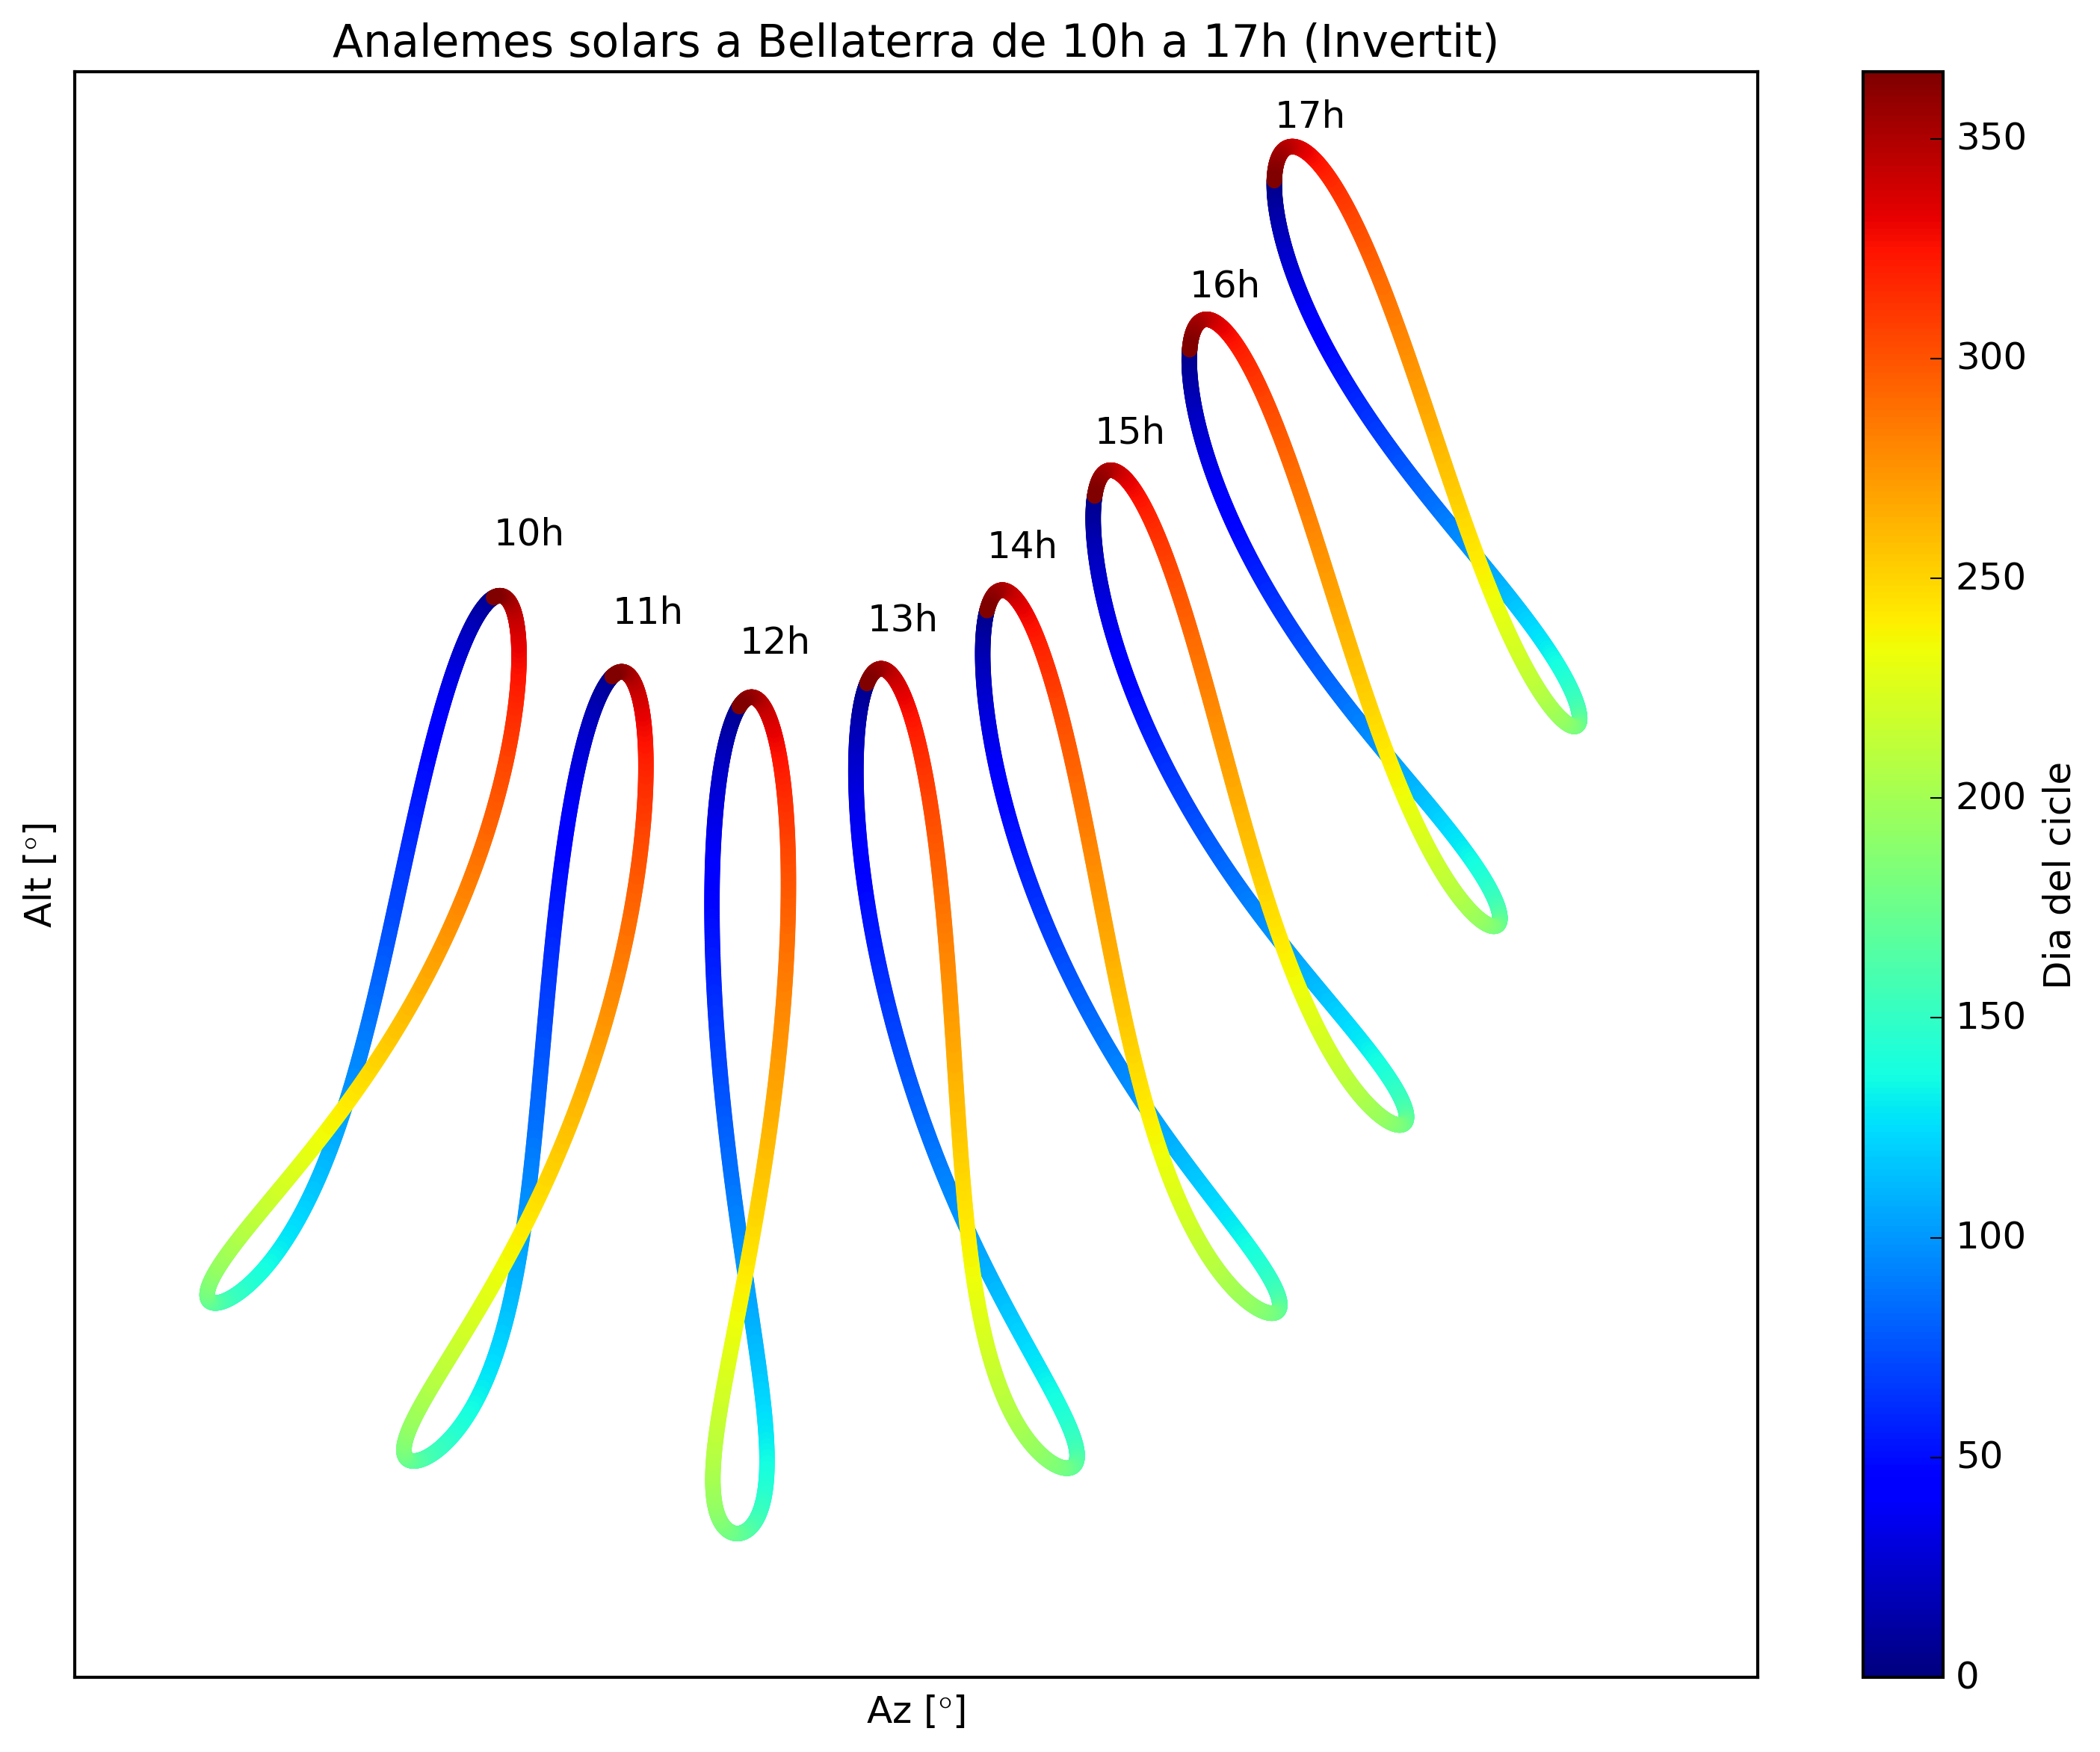
\includegraphics[width=\textwidth]{images/analema_simUAB_invert.png}
        \caption{Analemes (Invertint l'eix y) d'un conjunt d'hores vist des de la Terra. Font: Github del treball.}
        \label{subfig:analema_simUAB_invert}
    \end{subfigure}
\caption{Analemes solars vists des de Bellaterra des de les 10h fins les 17h}
\end{figure}
\vspace{2mm}

\noindent Com es pot observar, no s'asemblen molt el de la paret de la UAB i el graficat amb Python. Els 'loops' prims estàn localitzats a la part baixa dels analemes (En la figura de la UAB) mentre que, teóricament, s'observa que hauríen d'estar a la part alta. També, s'observa que els analemes de la UAB tenen una tendència a pujar en altitud mentre que els teórics disminueixen. Sembla ser que els analemes de la entrada de la UAB tenen l'eix vertical invertit i, si es fa aquesta transformació en els graficats teóricament amb Python, s'obté la figura \ref{subfig:analema_simUAB_invert}. Comparant la figura invertida amb els analemes de l'entrada de la UAB, es veu una correlació molt major. Igualment no són exactes, doncs els de la UAB tenen una tendencia a augmentar en declinació mentre que els teórics segueixen una corba amb un mínim. També, la inclinació dels analemes és diferent en ambdós figures. Sembla ser que els eixos no són dúes rectes perpendiculars, sinó que tenen una certa curvatura. Implementar un model que intenti replicar la figura seguint aquesta hipòtesi es complica doncs els eixos poden ser completament arbitraris, així doncs s'emprarà la figura invertida com la millor aproximació.

\vspace{2mm}

\noindent L'explicació del fet que els analemes observats a l'entrada de la UAB no segueixen la figura teoritzada prové del fet que, realment, la intenció de la figura no és representar els analemes a diverses hores. Aquest és un rellotge solar analemàtic, el qual utilitza la projecció adaptada a la paret vertical i al gnomon i combina diversos factors per poder llegir l'hora solar al llarg de tot l'any. Els analemes graficats segueixen un sistema de coordenades útils i, per tant, la hipòtesi final és correcta. Un anàlisi més detallat sobre els rellotges solars analèmatics i la utilitat dels analemes en aquests dispositius es pot trobar en l'exercici 8.

\vspace{2mm}

\noindent Per completitud, s'analitzen també els analemes teòrics de forma separada (figura \ref{subfig:analema_simUAB}). S'observa que l'analema corresponent a les 12h es presenta gairebé vertical i amb una alçada màxima respecte als altres. Això és coherent amb el fet que les 12h solars representen el migdia solar veritable, moment en què el Sol assoleix la seva màxima altitud al cel per a un dia determinat. Pel que fa a la inclinació dels altres analemes, es constata que: Per hores anteriors a les 12h, l'analema es desvia cap a azimuts menors (més cap a l'est) i, per hores posteriors a les 12h, es desvia cap a azimuts majors (més cap a l'oest). Aquest comportament reflecteix la variació diària del moviment aparent del Sol, així com l'efecte combinat de la declinació solar i la equació del temps en cada moment del dia.

\vspace{10mm}
\hrule\
\vspace{5mm}

%%%%%%%%%%%%%%%%%%%%%%%%%%%%%%%%%%%
%%%%%%%%%%%%%%%%%%%%%%%%%%%%%%%%%%%

\section*{EXERCICI 7}

\noindent Anem a comparar doncs si l'analema que s'ha generat en aquest treball és correcte. En l'aplicació d'ordinador Stellarium hi ha una opció d'executar scripts d'usuaris. Hi ha un script que genera un analema visual \cite{SCRIPT_STELLARIUM}. Cal recalcar que aquest script genera un analema solar a 2020, però, si en l'animació abans de que es generi l'analema cambiem la data, et genera l'analema pel 2025. La figura \ref{fig:analema_real} mostra l'analema generat per l'script en l'Stellarium.

\vspace{2mm}
FIG: analema real
\vspace{2mm}

\noindent Com es pot veure si es compara amb la figura \ref{fig:analema_alt}, ambdós analemas són, en esència, el mateix. Els dos es troben inclinats lleugerament cap a l'esquerra i tenen una forma de vuit. El loop superior és més prim i petit que el loop inferior. Els dos analemes tenen un màxim d'altitud per sobre dels $70 \degree$ i un mínim d'altitud per sota dels $30 \degree$. També, es pot observar que el analema de l'Stellarium està limitat en un azimut de $[175\degree ,185\degree]$ i, el generat propi, està limitat a $5 \degree$ per banda al voltant del meridià ón està centrat; ambdós límits són equivalents. Amb aquest anàlisi, es pot concloure que, aproximadament, són equivalents. 

\vspace{10mm}
\hrule\
\vspace{5mm}

%%%%%%%%%%%%%%%%%%%%%%%%%%%%%%%%%%%
%%%%%%%%%%%%%%%%%%%%%%%%%%%%%%%%%%%

\section*{EXERCICI 8}
\noindent Un rellotge solar ens marca l'hora solar aparent, mentre que els rellotges convencionals ens marquen l'hora solar mitjana. La diferència entre ambdós tipus de rellotges és la quantitat anomenada 'equació del temps' i està directament relacionada amb l'analema solar. Per mantenir el rellotge solar sincronitzat amb el temps solar mitjà, l'analema es pot utilitzar per corregir les fluctuacions causades per l'òrbita i la inclinació de la Terra. El patró de l'analema mostra on estaria el Sol a una hora específica de cada dia en comparació amb el temps solar mitjà.

\vspace{2mm}

\noindent A la pràctica, un rellotge solar pot tenir una escala o factor de correcció inscrit en ell, que ajusta la lectura segons la data. Per exemple, en certs dies, el rellotge solar podria mostrar una hora que estigui uns minuts avançada o endarrerida respecte al temps solar mitjà. En consultar l'analema (o una taula de l'Ecuació del Temps), es pot ajustar l'hora mostrada pel rellotge solar per fer que coincideixi amb el temps solar mitjà. Un exemple de rellotge solar amb correcció és el que es troba en la paret de la facultat de ciències de l'UAB. 
\vspace{10mm}
\hrule\
\vspace{5mm}

%%%%%%%%%%%%%%%%%%%%%%%%%%%%%%%%%%%
%%%%%%%%%%%%%%%%%%%%%%%%%%%%%%%%%%%

\section*{EXERCICI 9}

\noindent Finalment, per aquest últim apartat, s'intentarà observar la influència directa de l'inclinació de l'eix de rotació i l'excentricitat a l'hora de generar un analema. Per realitzar aquest anàlisi s'han proposat diversos planetes i s'ens demana de plotejar l'analema solar per cadascún d'ells. Les dades dels planetes es poden trobar en la taula \ref{tab:planetes}.

\vspace{2mm}
\begin{table}[h!]
    \centering
    \begin{tabular}{|c|c|c|}
        \hline
        Planeta & Obliqüitat [$\degree$] & Excentricitat $\epsilon$ \\
        \hline
        Mercuri & 0.03 & 0.21 \\
        Terra & 23.44 & 0.0167 \\
        Mart & 25.19 & 0.093 \\
        Júpiter & 3.13 & 0.0485 \\
        Saturn & 26.73 & 0.056 \\
        \hline
    \end{tabular}
    \caption{Dades dels planetes. Font: analemma.com \cite{PLANETES}.}
    \label{tab:planetes}
\end{table}
\vspace{2mm}

\noindent Per realitzar una bona comparativa, s'han generat els analemes per cada planeta i s'han comparat amb el observat si ens localitzem en el planeta en qüestió a l'Stellarium i augmentem els díes. A l'annex es poden trobar les gràfiques generades per cada planeta. Per realitzar aquest apartat s'ha escrit un nou script de Python que es pot trobar en el Github del treball. L'arxiu de l'script es diu $analema\_planetes.py$. El codi et calcula la declinació del sol a cada planeta, et calcula la diferència entre el temps solar mitjà i el temps solar aparent a partir d'una versió de l'equació del temps diferent a la de l'exercici 6 i, finalment, et grafica l'analema solar vist des de cadascún dels planetes. L'equació del temps utilitzada en aquest apartat és $EoT = M - ra$ (On $ra$ és l'ascensió recta del sol i $M$ és l'anomalia mitjana) i, ara, $M$ i $ra$ es troben emprant l'expressió exacta de l'exercici 4 truncada a 20 termes de la sèrie de Bessel. A més, s'ha obtingut la declinació i no s'ha emprat la llibreria ephem, ja que la llibreria et troba la declinació del sol vist des de la Terra. Aquests canvis es deuen a que és necesàri modificar els paràmetres de les òrbites planetàries i, per tant, no es pot emprar el codi $analema.py$.

\vspace{2mm}

\noindent Les órbites escullides són interessants doncs mostren una gran variació en l'excentricitat i l'inclinació i, per tant, el gran rang d'aspectes que es poden observar en un analema. Tenim 2 grans grups d'analemes segons la seva forma: analemes en forma de vuit (A la Terra, Mart o Saturn) i en forma elíptica (A Mercuri o Júpiter). Els planetes amb l'analema en forma de vuit tenen en comú una obliquitat alta ($\sim 25\degree$), mentre que els que tenen forma elíptica tenen una obliquitat molt baixa ($\sim 1\degree$). Amb aquesta observació es pot intuir la relació directa entre l'obliqüitat i l'accentuació del loop de l'analema. Com a exeple extrem, es pot observar Urà, que té una obliqüitat de $97.86 \degree$ i, si s'observa el seu analema, fa una forma de vuit extremadament accentuada. 

\vspace{2mm}

\noindent Per completitud, es finalitzarà aquest apartat amb el següent: Primer de tot, s'ha generat i analitzat un analema solar i, després, s'ha generalitzat el concepte d'analema a altres planetes (Doncs aquests també orbiten al voltant del sol); Finalment, es pot generalitzar el concepte d'analema a qualsevol cos celeste que orbiti al voltant d'un altre cos celeste. Com a exemple, es pot analitzar l'analema lunar, és a dir, l'analema de la luna vist des de la Terra. L'excentricitat de l'órbita Terra-Lluna és $\epsilon \approx 0.0549$ i, l'obliqüitat de l'órbita $\sim 6.68 \degree$ \cite{LLUNA}. La forma de l'analema lunar es pot trobar en la figura \ref{fig:analema_luna}.

\begin{figure}[h!]
    \centering
    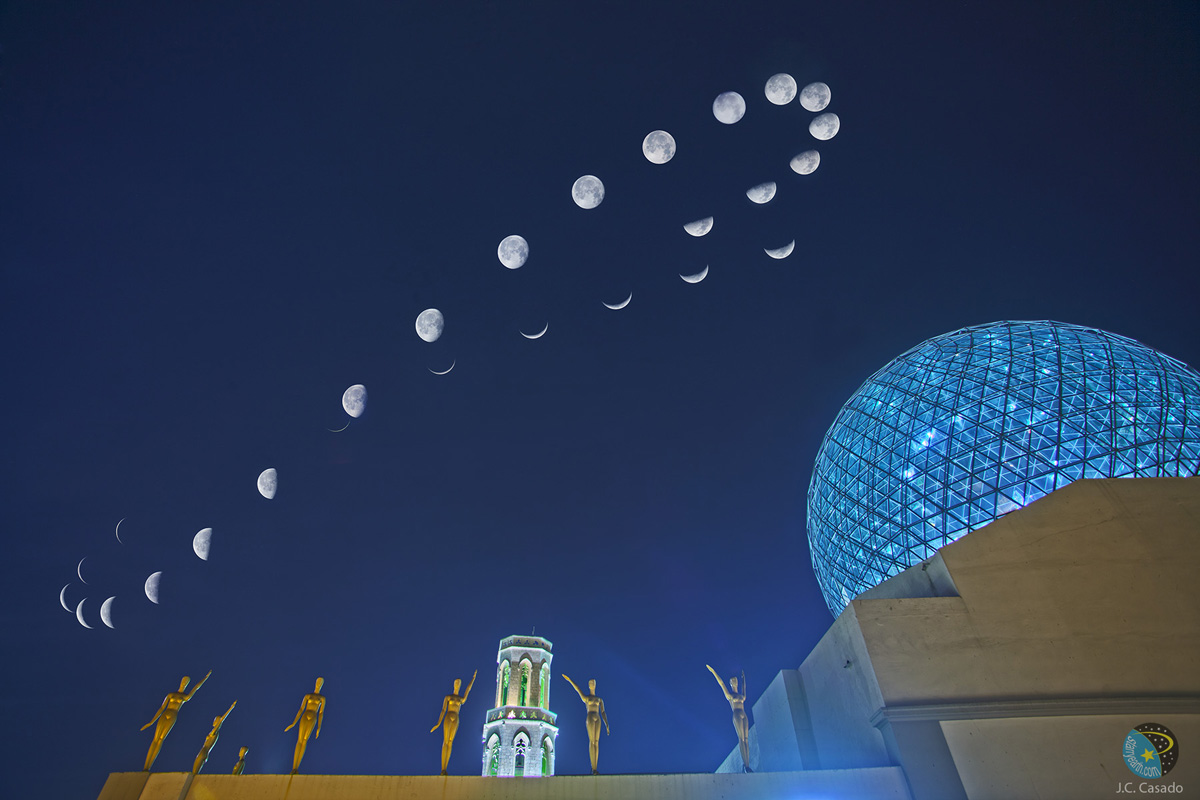
\includegraphics[width=0.55\textwidth]{images/analema_luna.jpg}
    \caption{Analema lunar vist des de la Terra. Font: TWANIGHT \cite{ANALEMA_MOON}.}
    \label{fig:analema_luna}
\end{figure}

\vspace{2mm}

\noindent Com es pot observar, la figura és la que es troba a l'anunciat de l'entrega. La imatge 'Lunar Analemma' és una composició fotogràfica que mostra el moviment de la Lluna sobre el Teatre-Museu Dalí de Figueres, Espanya, al llarg d'un mes lunar. Aquesta tècnica és similar a l'analema solar, però en aquest cas es realitza en un període de temps molt més curt (degut al fet que el període lunar és d'uns 27 dies, mentre que el solar és d'uns 365, aproximadament). Com es pot observar, la figura és coherent amb els analemes graficats anteriorment. L'órbita de la lluna té propietats similars a les de Júpiter, per tant, s'observa una figura allargada i inclinada també. A diferència de l'analema de Júpiter, aquesta té forma de vuit, però és probable doncs l'analema de Júpiter està bastant allargat i aprimat, per tant, pot ser que estigui a prop d'una obliqüitat que permet la formació del loop.


%\vspace{10mm}
%\hrule\
%\vspace{5mm}

%%%%%%%%%%%%%%%%%%%%%%%%%%%%%%%%%%%
%%%%%%%%%%%%%%%%%%%%%%%%%%%%%%%%%%%

\newpage
\section*{ANNEX}


%%%%%%%%%%%%%%%%%%%%%%%%%%%%%%%%%%%
%%%%%%%%%%%%%%%%%%%%%%%%%%%%%%%%%%%
%%%%%%%%%%%%%%%%%%%%%%%%%%%%%%%%%%%
%%%%%%%%%%%%%%%%%%%%%%%%%%%%%%%%%%%
%%%%%%%%%%%%%%%%%%%%%%%%%%%%%%%%%%%

\newpage
\printbibliography
\end{document}